%!TEX root = ../thesis.tex
%*******************************************************************************
%*********************************** First Chapter *****************************
%*******************************************************************************

\chapter{Introduction}  %Title of the First Chapter

\ifpdf
    \graphicspath{{Chapter1/Figs/Raster/}{Chapter1/Figs/PDF/}{Chapter1/Figs/}}
\else
    \graphicspath{{Chapter1/Figs/Vector/}{Chapter1/Figs/}}
\fi

\newcommand{\citetex}[1]{\citeauthor{#1} (\citeyear{#1})}
\newcommand{\citebrac}[1]{(\citeauthor{#1}, \citeyear{#1})}

%********************************** %Background  ****************************
\section{Background}

Casting bored piles and diaphragm walls in-situ ({\bfseries figure \ref{fig:tremie_blank}}) requires a specialist concrete termed 'tremie concrete'. In both fresh and cured state, this concrete must meet stringent design codes. Despite these regulations however, problems within the final product are still prevalent throughout the industry. In 2014 the European Federation of Foundation Contractors and the Deep Foundation Institute (USA) set up a task-group wherein the primary aim was to develop a clearer understanding of the root cause of these issues. The task group hypothesised that inadequate workability and stability of the concrete was, in part, caused by the inability of current design guidelines to predict when problems are likely to occur, \citetex{EFFC}.\\

\noindent
In order to provide evidence to support this hypothesis, two avenues of investigation have arisen. Namely, a practical approach as seen by \citet{bjorn}  and a simulative approach as described in this paper.\\

\noindent
Alongside an analysis of the issues to be investigated, a comprehensive review of literature surrounding fresh concrete and its ability to be modelled accurately is presented, followed by a potential methodology of investigation. 

\begin{figure}[H]
\centering
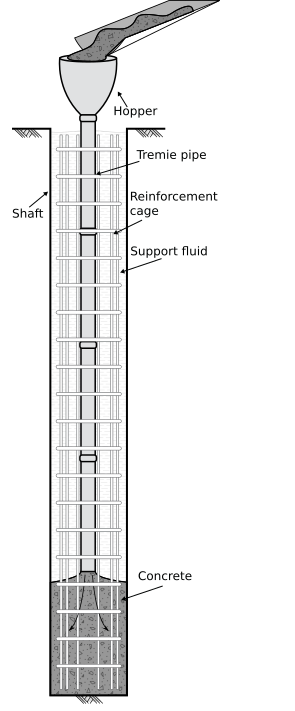
\includegraphics[width=0.6\textwidth]{tremie_empty.png}
\caption{\label{fig:tremie_blank} Schematic diagram of the tremie method for casting bored piles in situ.}
\end{figure}

\section{Research Objectives}
Coalescing all issues relating to tremie concrete into the same simulation is unlikely to produce any significant findings. A more pragmatic approach would be to assess each identified variable in the process individually, making a judgement it's impact on the final result.\\
\newline
\noindent
In this study, the impact of tremie method equipment shown in {\bfseries figure \ref{fig:tremie_blank}} is considered along side the resultant behaviour of the concrete, especially its dominant flow pattern. The change in behaviour of the concrete with changing variables will be documented in order to advise how best to avoid any issues that arise. Although there are some areas of investigation involving the tremie pipe, the dimensions and centring of the pipe as specified by EN 1536:2010 are not considered. \\
\newline
\noindent
When analysing the tremie method, each area of investigation falls within one of three subdivisions; initiation of concrete flow, during concrete flow, and bleed and segregation, {\bfseries figure \ref{fig:tremie_colour}}.
\begin{figure}[H]
\centering
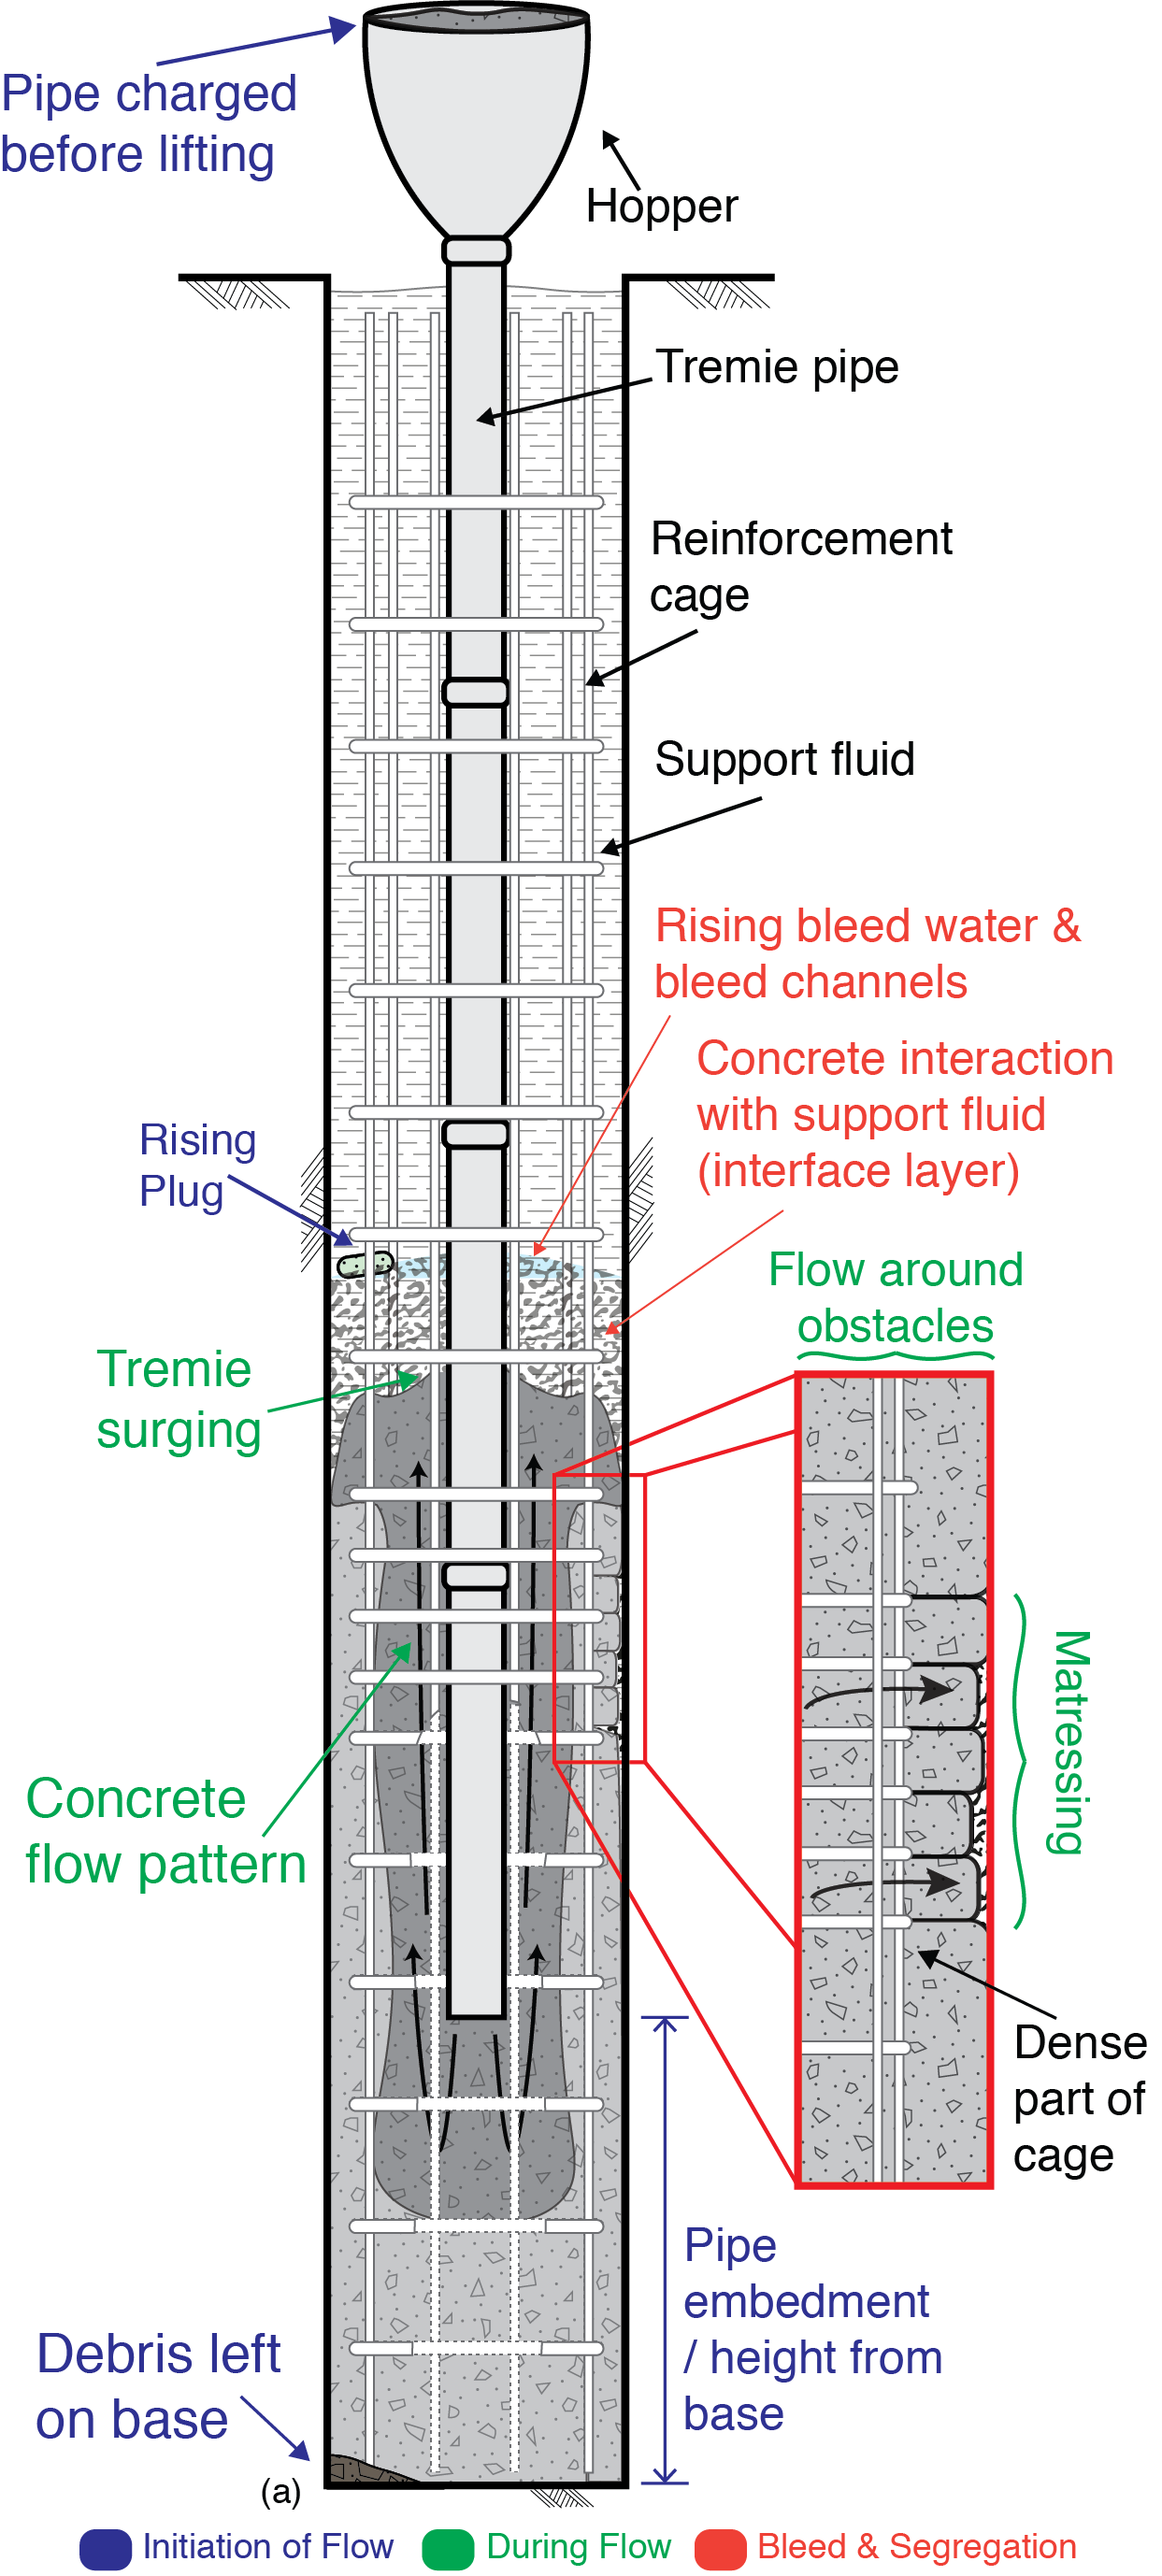
\includegraphics[width=0.6\textwidth]{combined_firstyear.png}
\caption{\label{fig:tremie_colour} Schematic diagram of a bored pile cast using tremie method, with areas of investigation highlighted and colour coded.}
\end{figure}









